% -*- TeX:de -*-
\NeedsTeXFormat{LaTeX2e}
\documentclass[12pt,a4paper,titlepage]{article}

%\usepackage[german]{babel} % german text
\usepackage[DIV12]{typearea} % size of printable area
\usepackage[T1]{fontenc} % font encoding
\usepackage[utf8]{inputenc} % probably on Linux

\usepackage{graphicx} % to include images
\graphicspath{ {img/} } % set default image directory
\usepackage{subfigure} % for creating subfigures
\usepackage{amsmath} % a bunch of symbols
\usepackage{amssymb} % even more symbols
\usepackage{booktabs} % pretty tables
\usepackage{csquotes}

% a floating environment for circuits
\usepackage{float}
\usepackage{caption}

\newfloat{circuit}{tbph}{circuits}
\floatname{circuit}{Schaltplan}

% a floating environment for diagrams
\newfloat{diagram}{tbph}{diagrams}
\floatname{diagram}{Diagramm}

\renewcommand{\familydefault}{\sfdefault} % activate to use sans-serif font as default

\sloppy % friendly typesetting

\usepackage{eurosym}
\usepackage{makeidx}
\usepackage{amsfonts}
\usepackage{mparhack}
\usepackage{array}
\usepackage{tabularx}
\usepackage{minitoc}
\usepackage[colorlinks=true]{hyperref}
\usepackage{epstopdf}
\usepackage{setspace}
\usepackage{csquotes}
\usepackage{circuitikz}

% hyperref settings
\hypersetup{
    colorlinks=false,       % false: boxed links; true: colored links
    linkcolor=black,          % color of internal links (change box color with linkbordercolor)
    citecolor=black,        % color of links to bibliography
    filecolor=black,      % color of file links
    urlcolor=black           % color of external links
}

\begin{document}

\begin{titlepage}

\begin{figure*}[h!]
  
\includegraphics[width=8cm]{TULogo_CMYK}
\end{figure*}

\begin{center}
\vspace*{1.3cm}
{\Huge Elektrotechnische Grundlagen der Informatik\\(LU 182.692)\\}
\vspace{1.7cm}
{\LARGE Protokoll der 4. Laborübung: \enquote{Spektren}\\}
\vspace{1.7cm}

% fill in group number and date of lab here
% CHANGE ME!
{\Large Gruppennr.: 22 \hspace{1cm} Datum der Labor\"ubung: 21.06.2017}

% fill in IDs and names here
% CHANGE ME!
\begin{table}[h!]
\centering
\begin{tabular}{|p{3.5cm}|p{3.5cm}|p{6.5cm}|}
\hline \textbf{Matr. Nr.} & \textbf{Kennzahl} & \textbf{Name} \\
\hline
1614835 & 033 535 & Jan Nausner \\
\hline
1633068 & 033 535 & David Pernerstorfer \\
\hline
\end{tabular}
\end{table}

\end{center}
\vspace{1.0cm}

\begin{table}[h!]
\begin{tabular}{|l|l|}
\hline \textbf{Kontrolle} & \checkmark \\
\hline Sinus-Signal im Frequenzbereich & \\
\hline Rechteck-Signal im Frequenzbereich & \\
\hline Amplitudenmodulation & \\
\hline Brückengleichrichter & \\
\hline
\end{tabular}
\end{table}

\end{titlepage}
% start of actual lab protocol
% CHANGE ME!

\setcounter{page}{2}

\newpage
\setcounter{tocdepth}{1}
\tableofcontents

\newpage

\section*{Materialien}
\begin{itemize}
	\item Oszilloskop: Agilent InfiniiVision MSO-X 3054A
	\item Frequenzgenerator: Agilent 33220A
  \item Netzteil Agilent U8031A
  \item Multimeter: Amprobe 37XR-A
\end{itemize}

\section{Messung eines Sinussignals im Spektralbereich mittels FFT}

\subsection*{Aufgabenstellung}

\subsection*{Schaltplan}
% \begin{figure}[H]
%   \centering
%   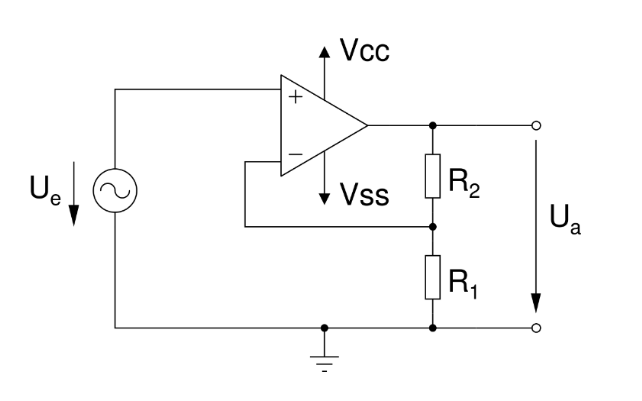
\includegraphics[width=100mm]{ni_opv_schaltung.png}
%   \caption{Nichtinvertierender OPV}
% \end{figure}

\subsection*{Durchf\"uhrung}

\subsection*{Ergebnisse \& Diskussion}


\section{Messung eines Rechtecksignals}

\subsection*{Schaltplan}
% \begin{figure}[H]
%   \centering
%   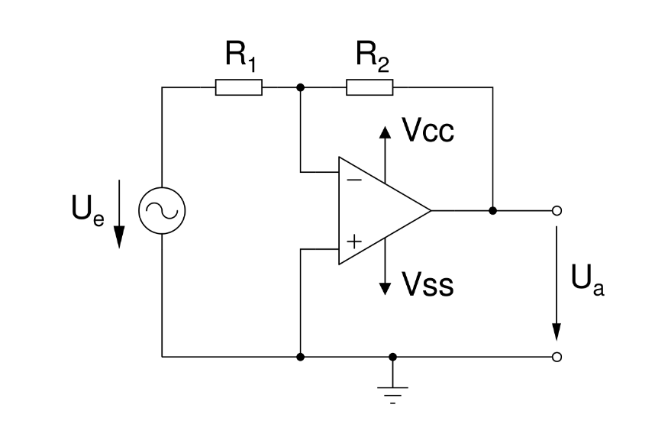
\includegraphics[width=100mm]{i_opv_schaltung.png}
%   \caption{Invertierender OPV}
% \end{figure}

\subsection*{Durchf\"uhrung}

\subsection*{Ergebnisse \& Diskussion}

\section{Amplitudenmodulation}

\subsection*{Aufgabenstellung}

\subsection*{Schaltplan}
% \begin{figure}[H]
%   \centering
%   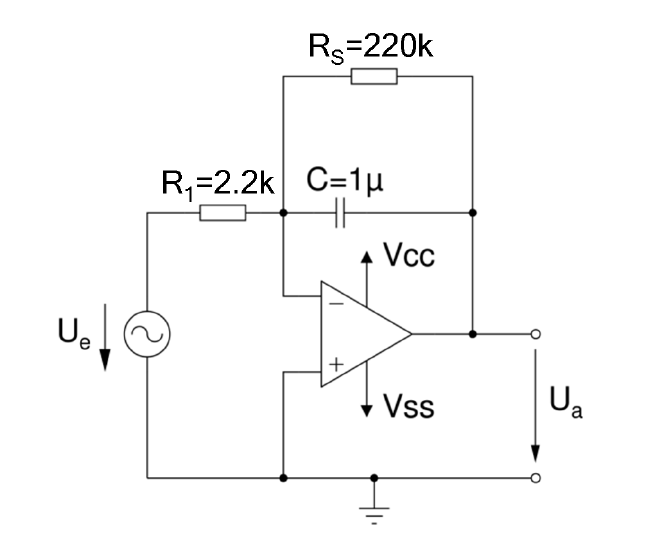
\includegraphics[width=80mm]{integrierer_opv_schaltung.png}
%   \caption{Integrierer}
%   \label{figure31}
% \end{figure}

\subsection*{Durchf\"uhrung}

\subsection*{Ergebnisse \& Diskussion}

\section{Brückengleichrichter}

\subsection*{Aufgabenstellung}

\subsection*{Schaltplan}
% \begin{figure}[H]
%   \centering
%   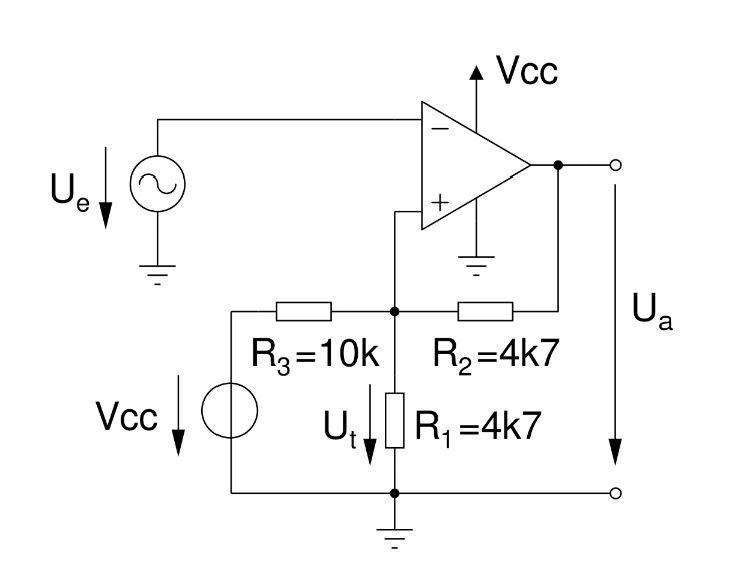
\includegraphics[width=80mm]{i_schmitt_trigger_schaltung.png}
%   \caption{Invertierender Schmitt-Trigger}
%   \label{figure41}
% \end{figure}


\subsection*{Durchf\"uhrung}

\newpage

\noindent Berechnung der Fourierreihe des gleichgerichteten Sinus:\\
\begin{align*}
    a_n &= \frac{2}{\pi}\int_{0}^{\pi}sin(t)\cdot cos(nt) dt\\
    &= \frac{1}{\pi}\int_{0}^{\pi}\left[sin(t - nt) + sin(t + nt)\right] dt\\
    &= \frac{1}{\pi}\left[\frac{1}{n-1}cos(t(1-n)) - \frac{1}{1+n}cos(t(1+n))\right]\bigr\rvert_{0}^{\pi}\\
    &= \frac{1}{\pi}\left[\frac{1}{n-1}cos(\pi-n\pi) - \frac{1}{1+n}cos(n\pi + \pi) - \frac{1}{n-1} + \frac{1}{1+n}\right]\\
    &= \frac{2cos(n\pi + \pi) - 2}{\pi(n+1)(n-1)} = \left\{
	    \begin{array}{ll}
		     0  & n \; ungerade \\
		     \frac{-4}{\pi(n+1)(n-1)} & n \; gerade
	    \end{array}
    \right.\\
    a_0 &= \frac{-4}{\pi(0+1)(0-1)} = \frac{4}{\pi}\\
    |sin(\omega t)| &= \frac{2}{\pi} - \sum_{n=1}^{\infty} \frac{4 \cdot cos(2n\omega t)}{\pi(2n+1)(2n-1)}
\end{align*}

\subsection*{Ergebnisse \& Diskussion}

\section{Anhang - Messwerte}

% \begin{figure}[H]
%   \centering
%   \begin{minipage}[b]{0.4\textwidth}
%     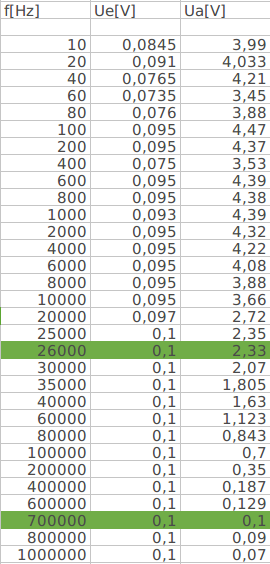
\includegraphics[width=\textwidth]{daten_471.png}
%     \caption{Messdaten invertierender OPV (-47 Verstärkung)}
%   \end{minipage}
%   \hfill
%   \begin{minipage}[b]{0.4\textwidth}
%     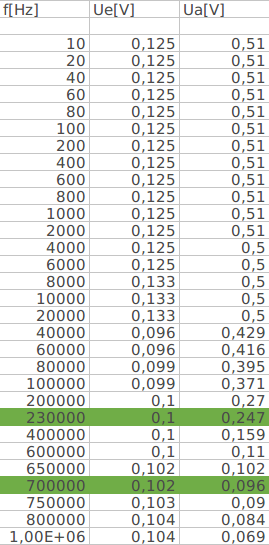
\includegraphics[width=\textwidth]{daten_4_7.png}
%     \caption{Messdaten invertierender OPV (-4,7 Verstärkung)}
%   \end{minipage}
% \end{figure}

\end{document}
